\documentclass[abstracton,12pt]{scrreprt}

\usepackage[utf8]{inputenc}
% \usepackage[T1]{fontenc}
\usepackage{fancyhdr}
\usepackage{graphicx}
\usepackage{tikz}
\usepackage{listings}
\usepackage{amssymb}
\usepackage{amsfonts}
\usepackage{amsmath}
\usepackage{pdfpages}
\usepackage{forest}
\usepackage{multicol}
\usepackage{varwidth}
\usepackage{verbatim}
\usepackage{cleveref}
\usepackage[ruled,vlined]{algorithm2e}

\forestset{qtree/.style={for tree={parent anchor=south, child anchor=north,align=left,inner sep=0pt}}}

% --------- 

\titlehead{Department of Informatics, University of Zürich}
\subject{\vspace*{2cm}BSc Vertiefungsarbeit}
\title{Detecting Volatile Index Nodes in a Hierarchical Database System}
\author{
  Rafael Kallis\\[-5pt]
  \scriptsize Matrikelnummer: 14-708-887\\[-5pt]
  \scriptsize Email: \texttt{rk@rafaelkallis.com}
}
\date{\vspace*{2cm}Oktober 3, 2017}
\publishers{
  \small supervised by Prof.\ Dr.\ Michael\ Böhlen and Kevin\ Wellenzohn \\[5cm]
  \begin{tikzpicture}[overlay]
    \node at (-3,-3) {
\includegraphics[height=1.5cm]{IFIlogo}};
    \node at (7,-3) {
\includegraphics[height=1.5cm]{dbtgBW}};
  \end{tikzpicture}
}

% \dedication{dedicated to xxx}

% --------- 

\newtheorem{definition}{Definition}
% \newtheorem{figure}{Figure}
% \newtheorem{example}{Example}
% \newtheorem{theorem}{Theorem}
% \newtheorem{lemma}{Lemma}

\crefname{algocfline}{alg.}{algs.}
\Crefname{algocfline}{Algorithm}{Algorithms}


% \newenvironment{proof}
%     {\noindent{\bf Proof:\rm}}{\hfill$\Box$\vspace{\medskipamount}}

\newenvironment{centerverbatim}{\par\centering\varwidth{\linewidth}\verbatim}
    {\endverbatim\endvarwidth\par}

\def\bbbr{{\rm I\!R}}
\def\bbbm{{\rm I\!M}}
\def\bbbn{{\rm I\!N}}
\def\bbbz{{\rm I\!Z}}

% --------- 

\begin{document}

\maketitle

% \chapter*{Acknowledgements}

% \begin{abstract}
%   ...
% \end{abstract}

% \chapter*{Zusammenfassung}

% \tableofcontents
% \listoffigures
% \listoftables

\chapter{INTRODUCTION}

Hierarchical indexes with skewed and update-heavy workloads grow and shrink often.
Since index modifications propagate up and down, adding and removing nodes cause a sequence of nodes to be added or removed in addition, thus deteriorating the index update performance.
Index update performance also suffers from conflicting index updates.
Highly skewed workloads create hotspots where nodes are frequently added or removed, increasing conflicting index updates, as shown in (ref kevin paper).

A content management system's workloads share common properties.
They are a) skewed and the same data item is repeatably added or removed from the index and
b) update-heavy.

Wellenzohn et al. (ref) propose a workload aware property index (WAPI). 
The WAPI exploits the workloads' skewness by not removing frequently accessed nodes from the PI.
By not removing these \textbf{volatile} nodes, we increase performance since we:
\begin{itemize}
    \item Reduce the amount of index modifications, which are expensive because they implicitly cause a sequence of nodes to be added or removed from the index.
    \item Decrease the number of index conflicts, which limit throughput since they cause a transaction to abort and restart.
\end{itemize}
An property index which can detect which nodes are volatile, is a \textbf{workload aware} property index (WAPI).

Apache Jackrabbit Oak (reference) (Oak) a hierarchical database system which makes use of a hierarchical index. 
Oak has two design goals in mind.
It needs to be able to operate in a distributed environment and guarantee write throughput.
Multiple Oak instances can work concurrently by making use of Multiversion Concurrency Control (MVCC) (reference), a commonly used optimistic technique (reference Principals of Distributed databases).
Whilst Oak is responsible for handling the database logic, it stores the actual data on MongoDB.
Although Oak is an open-source project, it is being actively maintained by Adobe (reference).
Adobe's content management system (CMS) makes use of Oak in one of their products, specifically Adobe Experience Manager.

The goal of this project is to implement a WAPI, as proposed by (ref kevin paper) in Apache Jackrabbit Oak in order to improve throughput.

\chapter{WAPI}

\section{Adding nodes to the WAPI}

Node $n$ is added to the WAPI iff $n$ has a property $k$ set to $v$.
Let's consider \cref{fig:add_wapi}.
Given snapshot $G^i$, transaction $T_j$ adds property \texttt{x} with value $1$ to \texttt{/a/b} and commits snapshot $G^j$.
The WAPI is updated as described in \cref{algo:add_triple_wapi}.

\begin{figure}[h]
    \begin{scriptsize}
        \begin{multicols}{2}
            \begin{large}
                $$ G^i \xrightarrow{\quad T_j \quad} G^j $$
            \end{large}
            \begin{multicols}{2}
                \begin{center}
                    \framebox(100,130){
                        \begin{forest} qtree,
                            [
                                [$\lambda:\texttt{index}$]
                                [,phantom]
                                [$\lambda:a$,name=a
                                    [,phantom]
                                    [$\lambda:b$,name=b]
                                    [,phantom]
                                    [$\lambda:c$]
                                ]
                            ]
                        \end{forest}
    
                        \vspace{27mm}
                    }
    
                    Snapshot $G^i$
                \end{center}
                \columnbreak
                \begin{center}
                    \framebox(100,130){
                        \begin{forest} qtree,
                            [
                                [$\lambda:\texttt{index}$
                                    [$\lambda:\texttt{x}$
                                        [$\lambda:\texttt{1}$
                                            [$\lambda:a$
                                            [$\lambda:b$ \\ $\texttt{x}:1$]
                                            ]
                                        ]
                                    ]
                                ]
                                [,phantom]
                                [$\lambda:a$,name=a
                                    [,phantom]
                                    [$\lambda:b$ \\ $\texttt{x}:\texttt{1}$,name=b]
                                    [,phantom]
                                    [$\lambda:c$]
                                ]
                            ]
                        \end{forest}
                    }
    
                    Snapshot $G^j$
                \end{center}    
            \end{multicols}
            \columnbreak
            \ 

            \vspace{12.2mm}
            \begin{algorithm}[H]
                \label{algo:add_triple_wapi}
                \caption{AddTripleWAPI}
                \DontPrintSemicolon
                \begin{scriptsize}
                    \KwData{Triple $(k, v, m)$, where $k$ is a property, $v$ a value and $m$ a node.}
                    \
                    
                    \vspace{1.2mm}
                    \Begin{
                        $n \longleftarrow \texttt{/index}$\;
                        \For{$\lambda \in \langle\, k,\, v,\, \dots\,,\, par(m)[\lambda],\, m[\lambda] \, \rangle$}{
                            $n \longleftarrow n | \texttt{/}\lambda$\;
                            \If{$\nexists n$}{
                                create node $n$\;
                            }
                        }
                        $n[k] \longleftarrow v$
                    }
                \end{scriptsize}
            \end{algorithm}

        \end{multicols}
    \end{scriptsize}
    \caption{Adding a node in a workload aware property index.}
    \label{fig:add_wapi}
\end{figure}

\section{Querying}

Oak mostly executes content-and-structure (CAS) queries \textbf{(ref)}.
Given node $m$, property $k$ and value $v$, a CAS query returns all descendants of $m$ which have $k$ set to the $v$.
An example of such a query can be found in \cref{fig:cas_query}.

\begin{definition}
    (CAS-Query): 
    {\large$Q_{k,v,m} = \{ \, n \, | \, n[k] = v \land n \in desc(m) \, \} $}
\end{definition}

\begin{figure}[h]
    \begin{multicols}{2}
        \begin{multicols}{2}
            \begin{center}
                \
                
                \begin{footnotesize}
                    \begin{forest} qtree,
                        [
                            [$\lambda:\texttt{index}$
                                [$\lambda:\texttt{x}$
                                    [$\lambda:\texttt{1}$
                                        [$\lambda:a$
                                        [$\lambda:b$ \\ $\texttt{x}:1$]
                                        ]
                                    ]
                                ]
                            ]
                            [,phantom]
                            [$\lambda:a$,name=a
                                [,phantom]
                                [$\lambda:b$ \\ $\texttt{x}:\texttt{1}$,name=b]
                                [,phantom]
                                [$\lambda:c$]
                            ]
                        ]
                    \end{forest}
                \end{footnotesize}
            \end{center}    
            \columnbreak
            \begin{footnotesize}
                \
                
                \vspace{5mm}
                Having the following query, that is every descendant of \texttt{/a} with \texttt{x} set to $1$,
                we receive a set including node \texttt{/a/b}.
            \end{footnotesize}
            \begin{large}
                $$ Q_{\texttt{x}, 1, \texttt{/a}} = \{\,\texttt{\normalsize/a/b}\,\}$$
            \end{large}
        \end{multicols}
        \columnbreak
        \begin{algorithm}[H]
            \DontPrintSemicolon
            \begin{scriptsize}
                \label{algo:query_pi}
                \caption{QueryPropertyIndex}
                \KwData{Triple $(k, v, m)$, where $k$ is a property, $v$ a value and $m$ a node.}
                \KwResult{$\{\,n \, | \, n[k] = v \land n \in desc(m) \, \}$}
                \Begin{
                    $n \longleftarrow \texttt{/index}$\;
                    \For{$\lambda \in \langle\, k,\, v,\, \dots\,,\, par(m)[\lambda],\, m[\lambda] \, \rangle$}{
                        $n \longleftarrow n | \texttt{/}\lambda$\;
                        \If{$\nexists n$}{
                            \Return{$\emptyset$}\;
                        }
                    }
                    $r \longleftarrow \emptyset$\;
                    \For{$d \in desc(n)$}{
                        \If{$d[k] = v$}{
                            $r \longleftarrow r \cup \{ trunc(d) \}$\;
                        }
                    }
                    \Return{r}\;
                }
            \end{scriptsize}
        \end{algorithm}
    \end{multicols}
    \caption{CAS Query example.}
    \label{fig:cas_query}
\end{figure}

\section{Removing nodes from the WAPI}

A workload aware property index differentiates itself from a property index mostly during node removal.
It detects which nodes are volatile and avoids removing them.
The process of classifying a node as volatile, will be explained in more details in \cref{sec:volatility}.

\Cref{fig:remove_wapi} depicts the following scenario.
Assume \texttt{/index/x/1/a/b} (colored red) is volatile in all three snapshots $G^i, G^j, G^k$.
Given snapshot $G^i$, transaction $T_j$ removes property \texttt{x} from \texttt{/a/b} and commits snapshot $G^j$.
Since \texttt{/index/x/1/a/b} is volatile, it is not removed from the WAPI.
Given snapshot $G^j$, transaction $T_k$ removes property \texttt{x} from \texttt{/a/c} and commits snapshot $G^k$.
Since \texttt{/index/x/1/a/b} is not volatile, it is removed from the WAPI.

\Cref{algo:remove_triple_wapi} describes the process of removing a node from the workload aware property index.

\begin{figure}[h]
    \begin{large}
        $$ G^i \xrightarrow{\quad T_j \quad} G^j \xrightarrow{\quad T_k \quad} G^k $$
    \end{large}
    \begin{scriptsize}
        \begin{multicols}{3}
            \begin{center}
                \framebox(130,130){
                    \begin{forest} qtree,
                        [
                            [$\lambda:\texttt{index}$
                                [$\lambda:\texttt{x}$
                                    [$\lambda:\texttt{1}$
                                        [$\lambda:a$
                                            [$\lambda:b$ \\ $\texttt{x}:1$, red]
                                            [,phantom]
                                            [,phantom]
                                            [$\lambda:c$ \\ $\texttt{x}:1$]
                                        ]
                                    ]
                                ]
                            ]
                            [,phantom]
                            [,phantom]
                            [,phantom]
                            [$\lambda:a$
                                [$\lambda:b$ \\ $\texttt{x}:\texttt{1}$]
                                [,phantom]
                                [$\lambda:c$ \\ $\texttt{x}:\texttt{1}$]
                            ]
                        ]
                    \end{forest}
                }

                Snapshot $G^i$
            \end{center}
            \columnbreak
            \begin{center}
                \framebox(130,130){
                    \begin{forest} qtree,
                        [
                            [$\lambda:\texttt{index}$
                                [$\lambda:\texttt{x}$
                                    [$\lambda:\texttt{1}$
                                        [$\lambda:a$
                                            [$\lambda:b$, red]
                                            [,phantom]
                                            [,phantom]
                                            [$\lambda:c$ \\ $\texttt{x}:1$]
                                        ]
                                    ]
                                ]
                            ]
                            [,phantom]
                            [,phantom]
                            [,phantom]
                            [$\lambda:a$
                                [$\lambda:b$]
                                [,phantom]
                                [$\lambda:c$ \\ $\texttt{x}:\texttt{1}$]
                            ]
                        ]
                    \end{forest}
                }

                Snapshot $G^j$
            \end{center}
            \columnbreak
            \begin{center}
                \framebox(130,130){
                    \begin{forest} qtree,
                        [
                            [$\lambda:\texttt{index}$
                                [$\lambda:\texttt{x}$
                                    [$\lambda:\texttt{1}$
                                        [$\lambda:a$
                                            [$\lambda:b$, red]
                                                [,phantom]
                                                [,phantom]
                                                [,phantom]
                                                [,phantom]
                                        ]
                                    ]
                                ]
                            ]
                            [,phantom]
                            [,phantom]
                            [,phantom]
                            [$\lambda:a$
                                [$\lambda:b$]
                                [,phantom]
                                [$\lambda:c$]
                            ]
                        ]
                    \end{forest}
                }

                Snapshot $G^k$
            \end{center}
        \end{multicols}
    \end{scriptsize}
    \caption{Removing a node from the WAPI. Assume \texttt{/index/x/1/a/b} (colored red) is volatile in all three snapshots $G^i, G^j, G^k$.}
    \label{fig:remove_wapi}
\end{figure}

\begin{algorithm}[H]
    \label{algo:remove_triple_wapi}
    \caption{RemoveTripleWAPI}
    \DontPrintSemicolon
    \begin{footnotesize}
        \KwData{Triple $(k, v, m)$, where $k$ is a property, $v$ a value and $m$ a node.}
        \Begin{
            $n \longleftarrow \texttt{/index/k/v/m}$\;
            $n[k] \longleftarrow \textsc{nil}$\;
            \While{$n[\lambda] \neq \texttt{index} \land chd(n) = \emptyset \land n[k] \neq v \land \textcolor{blue}{\lnot \ isVolatile(n)}$}{
                $u \longleftarrow n$\;
                $n \longleftarrow par(n)$\;
                remove node $u$\;
            }
        }
    \end{footnotesize}
\end{algorithm}

\section{Volatility}
\label{sec:volatility}

\begin{definition}
    (Volatile Node): node $n^j$ is volatile iff $n^j$'s volatility count (\cref{def:vol_count}) over history $H_i$ is greater or equal than the volatility threshold $\tau$, i.e
    \begin{large}$$ isVolatile(n^j, H_i) \iff vol(n^j, H_i) \geq \tau $$\end{large}
\end{definition}

\begin{definition}
    (Volatility Count): the number of times node $n^j$ was added or removed from snapshots contained in a sliding window of length $L$ over history $H_i$, i.e
    \begin{large}
        \begin{equation}
            \begin{split}
                vol(n^j, H_i) = | \{ G^b | \\
                & G^b \in H_i \land \\
                & t(G^b) \in [t_{n-L+1}, t_n] \land \\
                & \exists G^a[ G^a = pre(G^b, H_i) \land (\\
                & \quad n^a \notin N(G^a) \land n^b \in N(G^b) \lor \\ 
                & \quad n^a \in N(G^a) \land n^b \notin N(G^b) \\
                & )] \\
                \} |
            \end{split}
        \end{equation}
    \end{large}
    \label{def:vol_count}
\end{definition}

\begin{figure}
    \begin{large}
        $$ G^i \xrightarrow{\quad T_j \quad} G^j \xrightarrow{\quad T_k \quad} G^k \xrightarrow{\quad T_l \quad} G^l$$
    \end{large}
    \begin{scriptsize}
        \begin{multicols}{4}
            \begin{center}
                \framebox(100,130){
                    \begin{forest} qtree,
                        [
                            [$\lambda:\texttt{index}$
                                [$\lambda:\texttt{x}$
                                    [$\lambda:\texttt{1}$
                                        [$\lambda:a$
                                        [$\lambda:b$ \\ $\texttt{x}:1$]
                                        ]
                                    ]
                                ]
                            ]
                            [,phantom]
                            [$\lambda:a$,name=a
                                [,phantom]
                                [$\lambda:b$ \\ $\texttt{x}:\texttt{1}$,name=b]
                                [,phantom]
                                [$\lambda:c$]
                            ]
                        ]
                    \end{forest}
                }

                Snapshot $G^i$
            \end{center}
            \columnbreak
            \begin{center}
                \framebox(100,130){
                    \begin{forest} qtree,
                        [
                            [$\lambda:\texttt{index}$]
                            [,phantom]
                            [$\lambda:a$,name=a
                                [,phantom]
                                [$\lambda:b$,name=b]
                                [,phantom]
                                [$\lambda:c$]
                            ]
                        ]
                    \end{forest}

                    \vspace{27mm}
                }

                Snapshot $G^j$
            \end{center}
            \columnbreak
            \begin{center}
                \framebox(100,130){
                    \begin{forest} qtree,
                        [
                            [$\lambda:\texttt{index}$
                                [$\lambda:\texttt{x}$
                                    [$\lambda:\texttt{1}$
                                        [$\lambda:a$
                                        [$\lambda:b$ \\ $\texttt{x}:1$, red]
                                        ]
                                    ]
                                ]
                            ]
                            [,phantom]
                            [$\lambda:a$,name=a
                                [,phantom]
                                [$\lambda:b$ \\ $\texttt{x}:\texttt{1}$]
                                [,phantom]
                                [$\lambda:c$]
                            ]
                        ]
                    \end{forest}
                }

                Snapshot $G^k$
            \end{center}
            \columnbreak
            \begin{center}
                \framebox(100,130){
                    \
                    
                    \vspace{-24mm}
                    \begin{forest} qtree,
                        [
                            [$\lambda:\texttt{index}$
                                [$\lambda:\texttt{x}$
                                    [$\lambda:\texttt{1}$
                                        [$\lambda:a$
                                           [$\lambda:b$, red]
                                        ]
                                    ]
                                ]
                            ]
                            [,phantom]
                            [$\lambda:a$,name=a
                                [,phantom]
                                [$\lambda:b$,name=b]
                                [,phantom]
                                [$\lambda:c$]
                            ]
                        ]
                    \end{forest}

                    \vspace{27mm}
                }

                Snapshot $G^l$
            \end{center}
        \end{multicols}
    \end{scriptsize}
    Assume $\tau = 2$, $G^i,G^j,G^k,G^l \in H_i$ and $L$ has a value such that $G^i,G^j,G^k,G^l$ are in the sliding window.
    $n^i, n^j, n^k, n^l$ represent node \texttt{/index/x/1/a/b} in snapshots $G^i, G^j, G^k, G^l$ respectively.
    
    Given $G^i$, transaction $T_j$ removes property \texttt{x} from \texttt{/a/b} and commits $G^j$.
    
    Given $G^j$, transaction $T_k$ adds property \texttt{x} with value $1$ to \texttt{/a/b} and commits $G^k$.
    
    Given $G^k$, transaction $T_l$ removes property \texttt{x} from \texttt{/a/b} and commits $G^l$.
    
    Then:
    \begin{itemize}
        \item $vol(n^i, H_i) = 0$, \quad $isVolatile(n^i, H_i) = false$
        \item $vol(n^j, H_i) = 1$, \quad $isVolatile(n^j, H_i) = false$
        \item $vol(n^k, H_i) = 2$, \quad $isVolatile(n^k, H_i) = true$
        \item $vol(n^l, H_i) = 3$, \quad $isVolatile(n^l, H_i) = true$
    \end{itemize}    
    \caption{Volatility count changes with each snapshot.}
    \label{fig:vol_example}
\end{figure}

% In the following pages, we will take a closer look at Oak.
% Specifically, we will see how Oak handles querying, writing and concurrency control.
% After that we will describe an instance of a problem Oak is having and we will briefly introduce a solution which results in higher throughput under certain circumstances.
% Lastly, we will modify Oak's reference implementation in order to satisfy our solution.

% Since Oak's PI is hierarchical, its performance deteriorates if used with CMS' workloads.
% You can find application scenarios which demonstrate how the PI's performance suffers in \cref{sec:application_scenarios}.

















\newpage
\newpage

\chapter{Introduction}
 
% A content store is a database system which supports hierarchical (tree-structured) data.
% It behaves similarly to a traditional file system, that is, storing files/ data with metadata.
% Like common relational DBMSs, content stores also can provide transactions and querying.

Apache Jackrabbit Oak (reference) (Oak) a tree-structured database system, with two design goals in mind.
It needs to be able to \textbf{a)} \textit{operate in a distributed environment} and \textbf{b)} \textit{guarantee write throughput}.
Multiple Oak instances can work concurrently by making use of Multiversion Concurrency Control (MVCC) (reference), a commonly used optimistic technique (reference Principals of Distributed databases).
Whilst Oak is responsible for handling the database logic, it stores the actual data on MongoDB.
Although Oak is an Open-source project, it is being actively maintained by Adobe (reference).
Adobe's Content Management System (CMS) makes use of Oak in one of their products, specifically Adobe Experience Manager (AEM).

\begin{figure}[h]
    \centering
    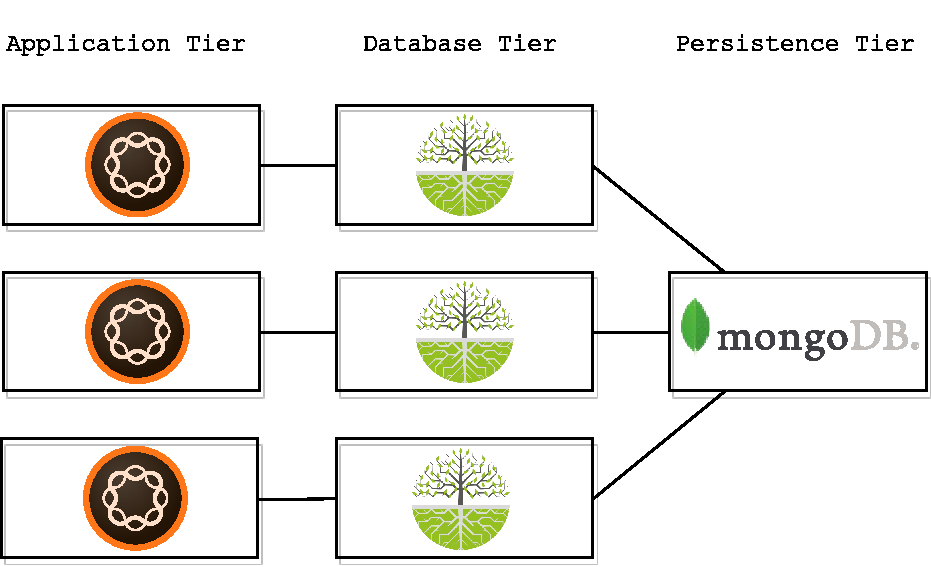
\includegraphics[width=8cm]{architecture}
    \caption{Apache Jackrabbit Oak's system architecture. The application, Adobe Experience Manage in this figure, connects to Oak.}
    \label{fig:architecture}
\end{figure}

In the following pages, we will take a closer look at Oak.
Specifically, we will see how Oak handles querying, writing and concurrency control.
After that we will describe an instance of a problem Oak is having and we will briefly introduce a solution which results in higher throughput under certain circumstances.
Lastly, we will modify Oak's reference implementation in order to satisfy our solution.

\chapter{Problem definition}

\section{Property Index}

Oak mostly executes content-and-structure (CAS) queries \textbf{(ref)}.
Given node $m$, property $k$ and value $v$, a CAS query returns all descendants of $m$ which have $k$ set to the $v$.
An example of such a query can be found in \cref{fig:cas_query}.

\begin{definition}
    (CAS-Query): 
    {\large$Q_{k,v,m} = \{ \, n \, | \, n[k] = v \land n \in desc(m) \, \} $}
\end{definition}

\begin{figure}[h]
    \begin{center}
        \begin{multicols}{2}
            \begin{forest} qtree,
                [
                    [,phantom]
                    [,phantom]
                    [$\lambda:\texttt{a}$
                        [$\lambda:\texttt{b}$ \\ $\texttt{x}:1$, draw]
                        [$\lambda:\texttt{c}$]
                    ]
                ]
            \end{forest}
            \columnbreak
            \begin{flushleft}
                Having the following query, that is every descendant of \texttt{/a} with \texttt{x} set to $1$,
                we receive a set including node \texttt{/a/b}, enclosed in a rectangle on the left.
            \end{flushleft}
            \begin{large}
                $$ Q_{\texttt{x}, 1, \texttt{/a}} = \{\,\texttt{\normalsize/a/b}\,\}$$
            \end{large}
        \end{multicols}
    \end{center}
    \caption{CAS Query example.}
    \label{fig:cas_query}
\end{figure}

In order to answer such queries efficiently, Oak implements a Property Index (PI) (ref kevin's paper).
A property index is a hierarchical index.
\Cref{fig:property_index} depicts a PI and shows how a CAS query can be answered by using it.
In addition to that you can find how a node is added or removed from the index.

% \newpage
\begin{figure}
    \begin{multicols}{2}
        \begin{center}(a) Tree with PI.\end{center}
        \vspace*{1px}
        \begin{center}

            \begin{forest} qtree,
                [
                    [$\lambda:\texttt{index}$
                        [$\lambda:\texttt{x}$
                            [$\lambda:\texttt{1}$
                                [$\lambda:a$
                                [$\lambda:b$ \\ $\texttt{x}:1$]
                                    [,phantom]
                                    [,phantom]
                                    [,phantom]
                                    [,phantom]
                                ]
                            ]
                        ]
                    ]
                    [,phantom]
                    [,phantom]
                    [,phantom]
                    [$\lambda:a$,name=a
                        [,phantom]
                        [,phantom]
                        [$\lambda:b$ \\ $\texttt{x}:\texttt{1}$,name=b]
                        [,phantom]
                        [$\lambda:c$]
                    ]
                ]
            \end{forest}
        \end{center}
        \columnbreak
        \begin{center}(b) Querying a tree with a PI.\end{center}
        \begin{algorithm}[H]
            \DontPrintSemicolon
            \begin{scriptsize}
                \label{algo:query_pi}
                \caption{QueryPropertyIndex}
                \KwData{Triple $(k, v, m)$, where $k$ is a property, $v$ a value and $m$ a node.}
                \KwResult{$\{\,n \, | \, n[k] = v \land n \in desc(m) \, \}$}
                \Begin{
                    $n \longleftarrow \texttt{/index}$\;
                    \For{$\lambda \in \langle\, k,\, v,\, \dots\,,\, par(m)[\lambda],\, m[\lambda] \, \rangle$}{
                        $n \longleftarrow n | \texttt{/}\lambda$\;
                        \If{$\nexists n$}{
                            \Return{$\emptyset$}\;
                        }
                    }
                    $r \longleftarrow \emptyset$\;
                    \For{$d \in desc(n)$}{
                        \If{$d[k] = v$}{
                            $r \longleftarrow r \cup \{ trunc(d) \}$\;
                        }
                    }
                    \Return{r}\;
                }
            \end{scriptsize}
        \end{algorithm}
    \end{multicols}
    \begin{multicols}{2}
        \begin{center}(c) Adding a node to the PI.\end{center}

        \begin{algorithm}[H]
            \label{algo:add_triple}
            \caption{AddTriple}
            \DontPrintSemicolon
            \begin{scriptsize}
                \KwData{Triple $(k, v, m)$, where $k$ is a property, $v$ a value and $m$ a node.}
                \vspace{2.2mm}
                \Begin{
                    $n \longleftarrow \texttt{/index}$\;
                    \For{$\lambda \in \langle\, k,\, v,\, \dots\,,\, par(m)[\lambda],\, m[\lambda] \, \rangle$}{
                        $n \longleftarrow n | \texttt{/}\lambda$\;
                        \If{$\nexists n$}{
                            create node $n$\;
                        }
                    }
                    $n[k] \longleftarrow v$
                }
            \end{scriptsize}
        \end{algorithm}
        \columnbreak
        \begin{center}(d) Removing a node from the PI.\end{center}

        \begin{algorithm}[H]
            \DontPrintSemicolon
            \begin{scriptsize}
                \label{algo:remove_triple_pi}
                \caption{RemoveTriple}
                \KwData{Triple $(k, v, m)$, where $k$ is a property, $v$ a value and $m$ a node.}
                \Begin{
                    $n \longleftarrow \texttt{/index/k/v/m}$\;
                    $n[k] \longleftarrow \textsc{nil}$\;
                    \While{$n[\lambda] \neq \texttt{index} \land chd(n) = \emptyset \land n[k] \neq v$}{
                        $u \longleftarrow n$\;
                        $n \longleftarrow par(n)$\;
                        remove node $u$\;
                    }
                }
            \end{scriptsize}
        \end{algorithm}
    \end{multicols}
    \begin{footnotesize}
        Where $\lambda$ is a node's label, i.e., node \texttt{/a/c} has \texttt{c} as a label,
        $|$ is the concatenation operator,
        $par(m)$ returns the parent node of $m$,
        $chd(n)$ returns the set of children nodes of $n$,
        $desc(n)$ returns the set of descendant nodes of $n$,
        $d[k]$ is the value of property $k$ of node $d$
        and $trunc(\texttt{/k/v/a/b}) = \texttt{/a/b}$ truncates the property name and value from the node.
    \end{footnotesize}
    \caption{Answering CAS queries efficiently using a Property Index.}
    \label{fig:property_index}
\end{figure}

\section{Workload implications}

A Content management system's workloads share common properties.
They are \textbf{a)} \textit{skewed and the same data item is repeatably added or removed from the index} and
\textbf{b)} \textit{update-heavy}.

Hierarchical indexes with skewed and update-heavy workloads grow and shrink often.
Since index modifications propagate up and down, adding and removing nodes cause a sequence of nodes to be added or removed in addition, thus deteriorating the index update performance, as shown in \cref{fig:update_pi}.
Index update performance also suffers from conflicting index updates.
Highly skewed workloads create hotspots where nodes are frequently added or removed, increasing conflicting index updates, as shown in (ref kevin paper).

Since Oak's PI is hierarchical, its performance deteriorates if used with CMS' workloads.
You can find application scenarios which demonstrate how the PI's performance suffers in \cref{sec:application_scenarios}.

\section{Proposal}

In order to improve performance, the following is being proposed.
We exploit the workloads' skewness by not removing frequently accessed nodes from the PI.
By not removing these \textbf{volatile} nodes, we:
\begin{itemize}
    \item Trade query performance for update performance.
    \item Decrease the number of index conflicts thus increasing update performance.
\end{itemize}
A property index which can detect which nodes are volatile, is a \textbf{workload aware} property index (WAPI).
A WAPI removes nodes as shown in \cref{algo:remove_triple_wapi}.
Besides checking if a node is volatile, \cref{algo:remove_triple_wapi} shares no other differences in comparison with \cref{algo:remove_triple_pi}.

% \begin{algorithm}
%     \label{algo:remove_triple_wapi}
%     \caption{RemoveTripleWAPI}
%     \DontPrintSemicolon
%     \begin{footnotesize}
%         \KwData{Triple $(k, v, m)$, where $k$ is a property, $v$ a value and $m$ a node.}
%         \Begin{
%             $n \longleftarrow \texttt{/index/k/v/m}$\;
%             $n[k] \longleftarrow \textsc{nil}$\;
%             \While{$n[\lambda] \neq \texttt{index} \land chd(n) = \emptyset \land n[k] \neq v \land \textcolor{blue}{\lnot \ isVolatile(n)}$}{
%                 $u \longleftarrow n$\;
%                 $n \longleftarrow par(n)$\;
%                 remove node $u$\;
%             }
%         }
%     \end{footnotesize}
% \end{algorithm}

\chapter{Application Scenarios}
\label{sec:application_scenarios}

\section{Tree growing and shrinking.}

Let's consider \cref{fig:update_pi}.
The tree in \cref{fig:update_pi} has a property index which is not workload aware.

Transaction $T_1$ removes property \texttt{x} from \texttt{/a/b}.
\texttt{x} is removed from  \texttt{/index/x/1/a/b}.
In addition to that, all ancestor nodes, $ anc(\texttt{/index/x/1/a/b}) = \{ \texttt{/index/x}, \texttt{/index/x/1}, \texttt{/index/x/1/a} \} \subset G^0, $ are removed as well. (c.f \cref{algo:remove_triple_pi})

Transaction $T_2$ adds property \texttt{x} to \texttt{/a/b}.
We first have to add all ancestors in order to add \texttt{/index/x/1/a/b} to the property index (c.f \cref{algo:add_triple}).

\begin{figure}[h]
    \begin{large}
        $$ G^0 \xrightarrow{\quad T_1 \quad} G^1 \xrightarrow{\quad T_2 \quad} G^2 $$
    \end{large}
    \begin{scriptsize}
        \begin{multicols}{3}
            \begin{center}
                \framebox(130,130){
                    \begin{forest} qtree,
                        [
                            [$\lambda:\texttt{index}$
                                [$\lambda:\texttt{x}$
                                    [$\lambda:\texttt{1}$
                                        [$\lambda:a$
                                        [$\lambda:b$ \\ $\texttt{x}:1$]
                                            [,phantom]
                                            [,phantom]
                                            [,phantom]
                                            [,phantom]
                                        ]
                                    ]
                                ]
                            ]
                            [,phantom]
                            [,phantom]
                            [,phantom]
                            [$\lambda:a$,name=a
                                [,phantom]
                                [,phantom]
                                [$\lambda:b$ \\ $\texttt{x}:\texttt{1}$,name=b]
                                [,phantom]
                                [$\lambda:c$]
                            ]
                        ]
                    \end{forest}
                }

                Tree $G^0$
            \end{center}
            \columnbreak
            \begin{center}
                \framebox(130,130){
                    \begin{forest} qtree,
                        [
                            [$\lambda:\texttt{index}$]
                            [,phantom]
                            [,phantom]
                            [,phantom]
                            [$\lambda:a$,name=a
                                [,phantom]
                                [,phantom]
                                [$\lambda:b$,name=b]
                                [,phantom]
                                [$\lambda:c$]
                            ]
                        ]
                    \end{forest}

                    \vspace{27mm}
                }

                Tree $G^1$
            \end{center}
            \columnbreak
            \begin{center}
                \framebox(130,130){
                    \begin{forest} qtree,
                        [
                            [$\lambda:\texttt{index}$
                                [$\lambda:\texttt{x}$
                                    [$\lambda:\texttt{1}$
                                        [$\lambda:a$
                                        [$\lambda:b$ \\ $\texttt{x}:1$]
                                            [,phantom]
                                            [,phantom]
                                            [,phantom]
                                            [,phantom]
                                        ]
                                    ]
                                ]
                            ]
                            [,phantom]
                            [,phantom]
                            [,phantom]
                            [$\lambda:a$,name=a
                                [,phantom]
                                [,phantom]
                                [$\lambda:b$ \\ $\texttt{x}:\texttt{1}$,name=b]
                                [,phantom]
                                [$\lambda:c$]
                            ]
                        ]
                    \end{forest}
                }

                Tree $G^2$
            \end{center}
        \end{multicols}
    \end{scriptsize}
    \caption{Updating a node in a property index.}
    \label{fig:update_pi}
\end{figure}

\Cref{fig:update_wapi} depicts the same transactions but the property index is workload aware.
Assume \texttt{/index/x/1/a/b} is volatile in all .
Transaction $T_1$ removes property \texttt{x} from \texttt{/a/b}.
\texttt{x} is removed from \texttt{/index/x/1/a/b} but since it is volatile, the node is not removed from the WAPI (c.f \cref{algo:remove_triple_wapi}).
This avoids removal of its ancestors.
Transaction $T_2$ adds property \texttt{x} to \texttt{/a/b}.
Since \texttt{/index/x/1/a/b} is volatile, it already exists in the WAPI along with its ancestors.
This avoided adding its ancestors.

\begin{figure}[h]
    \begin{large}
        $$ G^0 \xrightarrow{\quad T_1 \quad} G^1 \xrightarrow{\quad T_2 \quad} G^2 $$
    \end{large}
    \begin{scriptsize}
        \begin{multicols}{3}
            \begin{center}
                \framebox(130,130){
                    \begin{forest} qtree,
                        [
                            [$\lambda:\texttt{index}$
                                [$\lambda:\texttt{x}$
                                    [$\lambda:\texttt{1}$
                                        [$\lambda:a$
                                        [$\lambda:b$ \\ $\texttt{x}:1$]
                                            [,phantom]
                                            [,phantom]
                                            [,phantom]
                                            [,phantom]
                                        ]
                                    ]
                                ]
                            ]
                            [,phantom]
                            [,phantom]
                            [,phantom]
                            [$\lambda:a$,name=a
                                [,phantom]
                                [,phantom]
                                [$\lambda:b$ \\ $\texttt{x}:\texttt{1}$,name=b]
                                [,phantom]
                                [$\lambda:c$]
                            ]
                        ]
                    \end{forest}
                }

                Tree $G^0$
            \end{center}
            \columnbreak
            \begin{center}
                \framebox(130,130){
                    \begin{forest} qtree,
                        [
                            [$\lambda:\texttt{index}$
                                [$\lambda:\texttt{x}$
                                    [$\lambda:\texttt{1}$
                                        [$\lambda:a$
                                        [$\lambda:b$\\\ ]
                                            [,phantom]
                                            [,phantom]
                                            [,phantom]
                                            [,phantom]
                                        ]
                                    ]
                                ]
                            ]
                            [,phantom]
                            [,phantom]
                            [,phantom]
                            [$\lambda:a$,name=a
                                [,phantom]
                                [,phantom]
                                [$\lambda:b$,name=b]
                                [,phantom]
                                [$\lambda:c$]
                            ]
                        ]
                    \end{forest}
                }

                Tree $G^1$
            \end{center}
            \columnbreak
            \begin{center}
                \framebox(130,130){
                    \begin{forest} qtree,
                        [
                            [$\lambda:\texttt{index}$
                                [$\lambda:\texttt{x}$
                                    [$\lambda:\texttt{1}$
                                        [$\lambda:a$
                                        [$\lambda:b$ \\ $\texttt{x}:1$]
                                            [,phantom]
                                            [,phantom]
                                            [,phantom]
                                            [,phantom]
                                        ]
                                    ]
                                ]
                            ]
                            [,phantom]
                            [,phantom]
                            [,phantom]
                            [$\lambda:a$,name=a
                                [,phantom]
                                [,phantom]
                                [$\lambda:b$ \\ $\texttt{x}:\texttt{1}$,name=b]
                                [,phantom]
                                [$\lambda:c$]
                            ]
                        ]
                    \end{forest}
                }

                Tree $G^2$
            \end{center}
        \end{multicols}
    \end{scriptsize}
    \caption{Updating a volatile node in a workload aware property index. Assume \texttt{/index/x/1/a/b} is volatile.}
    \label{fig:update_wapi}
\end{figure}

\section{Index conflicts}

Although two concurrent transactions may have conflicts, some conflicts are \textbf{avoidable}.
Transactions $T_1$ and $T_2$ have an avoidable conflict iff $T_1$ and $T_2$ have a conflict and all conflicting nodes are nodes in the property index.
(kevin's paper) describes extensively when two transactions have a conflict.
\Cref{fig:index_conflict_pi} depicts an avoidable index conflict in a non workload aware PI.
Assume $T_1$ committed before $T_2$. Since Oak uses a first committer wins strategy, $T_2$ is forced to abort and restart

\begin{figure}[h]
    \begin{large}
        $$ G^0 \xrightarrow{\quad T_1 \quad} G^1 $$ $$ G^0 \xrightarrow{\quad T_2 \quad} G^2 $$
    \end{large}
    \begin{scriptsize}
        \begin{multicols}{3}
            \begin{center}
                \framebox(130,130){
                    \begin{forest} qtree,
                        [
                            [$\lambda:\texttt{index}$
                                [$\lambda:\texttt{x}$
                                    [$\lambda:\texttt{1}$
                                        [$\lambda:a$
                                        [$\lambda:b$ \\ $\texttt{x}:1$]
                                            [,phantom]
                                            [,phantom]
                                            [,phantom]
                                            [,phantom]
                                        ]
                                    ]
                                ]
                            ]
                            [,phantom]
                            [,phantom]
                            [,phantom]
                            [$\lambda:a$,name=a
                                [,phantom]
                                [,phantom]
                                [$\lambda:b$ \\ $\texttt{x}:\texttt{1}$,name=b]
                                [,phantom]
                                [$\lambda:c$]
                            ]
                        ]
                    \end{forest}
                }

                Tree $G^0$
            \end{center}
            \columnbreak
            \begin{center}
                \framebox(130,130){
                    \begin{forest} qtree,
                        [
                            [$\lambda:\texttt{index}$]
                            [,phantom]
                            [,phantom]
                            [,phantom]
                            [$\lambda:a$,name=a
                                [,phantom]
                                [,phantom]
                                [$\lambda:b$,name=b]
                                [,phantom]
                                [$\lambda:c$]
                            ]
                        ]
                    \end{forest}

                    \vspace{27mm}
                }

                Tree $G^1$
            \end{center}
            \columnbreak
            \begin{center}
                \framebox(130,130){
                    \begin{forest} qtree,
                        [
                            [$\lambda:\texttt{index}$
                                [$\lambda:\texttt{x}$
                                    [$\lambda:\texttt{1}$
                                        [$\lambda:a$
                                            [$\lambda:b$ \\ $\texttt{x}:1$]
                                            [,phantom]
                                            [,phantom]
                                            [,phantom]
                                            [,phantom]
                                            [$\lambda:c$ \\ $\texttt{x}:1$]
                                        ]
                                    ]
                                ]
                            ]
                            [,phantom]
                            [,phantom]
                            [,phantom]
                            [$\lambda:a$,name=a
                                [,phantom]
                                [,phantom]
                                [$\lambda:b$ \\ $\texttt{x}:\texttt{1}$,name=b]
                                [,phantom]
                                [$\lambda:c$ \\ $\texttt{x}:\texttt{1}$,name=c]
                            ]
                        ]
                    \end{forest}
                }

                Tree $G^2$
            \end{center}
        \end{multicols}
    \end{scriptsize}
    \caption{Index conflict in the property index.}
    \label{fig:index_conflict_pi}
\end{figure}

\begin{figure}[h]
    \begin{large}
        $$ G^0 \xrightarrow{\quad T_1 \quad} G^1 $$ $$ G^0 \xrightarrow{\quad T_2 \quad} G^2 $$
    \end{large}
    \begin{scriptsize}
        \begin{multicols}{3}
            \begin{center}
                \framebox(130,130){
                    \begin{forest} qtree,
                        [
                            [$\lambda:\texttt{index}$
                                [$\lambda:\texttt{x}$
                                    [$\lambda:\texttt{1}$
                                        [$\lambda:a$
                                        [$\lambda:b$ \\ $\texttt{x}:1$]
                                            [,phantom]
                                            [,phantom]
                                            [,phantom]
                                            [,phantom]
                                        ]
                                    ]
                                ]
                            ]
                            [,phantom]
                            [,phantom]
                            [,phantom]
                            [$\lambda:a$,name=a
                                [,phantom]
                                [,phantom]
                                [$\lambda:b$ \\ $\texttt{x}:\texttt{1}$,name=b]
                                [,phantom]
                                [$\lambda:c$]
                            ]
                        ]
                    \end{forest}
                }

                Tree $G^0$
            \end{center}
            \columnbreak
            \begin{center}
                \framebox(130,130){
                    \begin{forest} qtree,
                        [
                            [$\lambda:\texttt{index}$
                                [$\lambda:\texttt{x}$
                                    [$\lambda:\texttt{1}$
                                        [$\lambda:a$
                                        [$\lambda:b$\\\ ]
                                            [,phantom]
                                            [,phantom]
                                            [,phantom]
                                            [,phantom]
                                        ]
                                    ]
                                ]
                            ]
                            [,phantom]
                            [,phantom]
                            [,phantom]
                            [$\lambda:a$,name=a
                                [,phantom]
                                [,phantom]
                                [$\lambda:b$,name=b]
                                [,phantom]
                                [$\lambda:c$]
                            ]
                        ]
                    \end{forest}
                }

                Tree $G^1$
            \end{center}
            \columnbreak
            \begin{center}
                \framebox(130,130){
                    \begin{forest} qtree,
                        [
                            [$\lambda:\texttt{index}$
                                [$\lambda:\texttt{x}$
                                    [$\lambda:\texttt{1}$
                                        [$\lambda:a$
                                            [$\lambda:b$ \\ $\texttt{x}:1$]
                                            [,phantom]
                                            [,phantom]
                                            [,phantom]
                                            [,phantom]
                                            [$\lambda:c$ \\ $\texttt{x}:1$]
                                        ]
                                    ]
                                ]
                            ]
                            [,phantom]
                            [,phantom]
                            [,phantom]
                            [$\lambda:a$,name=a
                                [,phantom]
                                [,phantom]
                                [$\lambda:b$ \\ $\texttt{x}:\texttt{1}$,name=b]
                                [,phantom]
                                [$\lambda:c$ \\ $\texttt{x}:\texttt{1}$,name=c]
                            ]
                        ]
                    \end{forest}
                }

                Tree $G^2$
            \end{center}
        \end{multicols}
    \end{scriptsize}
    \caption{Avoided index conflict in the workload aware property index. Assume \texttt{/index/x/1/a/b} is volatile.}
    \label{fig:index_conflict_wapi}
\end{figure}
































\chapter{Oak's Mechanics}

\section{Persistence Tier}

Before we get into the inner workings of Oak, we need to understand how Oak chose to persist data.
As mentioned earlier, Oak's data is tree-structured and is stored in a MongoDB instance.
Each tree node is persisted in the shape of a JSON document.
Each tree node contains properties, which are represented by key-value pairs inside the JSON document.
Each node is identifiable by its tree-depth concatenated with its absolute path from the root node, denoted as \texttt{"\_id"}, which is also a unique identifier.
\Cref{fig:tree_and_json} illustrates a tree alongside its persisted state.

\begin{figure}
    \centering
    \begin{multicols}{3}
        \begin{forest}
            [, circle, draw
                [,phantom]
                [$\lambda:\texttt{a}$
                    [$\lambda:\texttt{b}$]
                    [$\lambda:\texttt{c}$]
                ]
            ]
        \end{forest}
        \footnotesize
        \begin{centerverbatim}
[
    { "_id": "0:/",    /* ... */ },
    { "_id": "1:/a",   /* ... */ },
    { "_id": "2:/a/b", /* ... */ },
    { "_id": "2:/a/c", /* ... */ }
]
        \end{centerverbatim}
    \end{multicols}
    \caption{A tree and its JSON representation.}
    \label{fig:tree_and_json}
\end{figure}

\begin{figure}
    \scriptsize
    \begin{centerverbatim}
[
    {
        "_id": "2:/a/c", 
        "x": {
            "r15ca9f191c0-0-1": "1",
            "r15cabff1500-0-2": "2",
            "r15cac0dbb00-0-2": "3"
        },
        "_deleted": {
            "r15ca9eb2920": false,      /* added */
            "r15ca9ec1380": true,       /* removed */
            "r15ca9ecfde0-0-1": false   /* added */
        },
        /* ... */
    },
    /* ... */
]
    \end{centerverbatim}
    \caption{A node's property in detail.}
    \label{fig:node_property}
\end{figure}

In order to support MVCC, Oak keeps a history of values each property had in the past such that we are able to tell when each value was persisted and which Oak instance committed the change. 
Properties which have such a history are called versioned properties.
In \cref{fig:node_property}, we take a look at node \texttt{/a/c} and see how property \texttt{x}'s value changes over time.

Oak also keeps a versioned property in order to determine if a node was added or deleted.
The property is called \texttt{"\_deleted"} and has a boolean value.

Each value's key is composed with a timestamp, a counter that is used to differentiate between value changes during the same instance of time and the identifier of the oak instance committing the change.
Let's consider \texttt{r15cac0dbb00-0-2}.
\texttt{r} is a standard prefix and can be neglected.
The \texttt{15cac0dbb00} following \texttt{r}, is an timestamp (number of milliseconds since the Epoch) in hexadecimal encoding which represents the time during which the change was committed.
The \texttt{0} following the timestamp, tells that the change was the 1st change of the specific property during that instance of time.
The \texttt{2} following the counter, tells that the change was committed by the Oak instance with an id of \texttt{2}.

It is worth mentioning that certain properties exist which are not meant for public usage.
Such values are prefixed with an underscore (\texttt{\_}).

\section{Periodic Synchronization}

Even though every cluster node $O_i$ accesses the same MongoDB instance,
each $O_i$ sees a different slice of MongoDB.
Every $O_i$ performs periodic synchronization with the MongoDB instance.
During the synchronization, the cluster node:
\begin{enumerate}
    \item Makes locally committed changes visible to other cluster nodes.
    \item Gains access to changes other cluster nodes have made visible.
\end{enumerate}

The synchronization is executed on a background process and is independent from the transactions.
In the following chapter, we will see how synchronization works in more detail.
Specifically, making locally committed changes visible (1) is covered in {\huge{cref\{transaction-write\}}\par} and
gaining access to new changes (2) is covered in \cref{transaction-read}.

\section{Transactions}

In this chapter we will see how Oak handles transactions.
Since Oak has to operate in a distributed environment, the underlying data structure is immutable in order to prevent side-effect and keep Oak thread-safe (reference oak).
Specifically, Oak implements a Persistent Tree (reference cormen).
A transaction is composed as follows:

$$
Read \longrightarrow Validate \longrightarrow Write
$$

\subsection{Read} \label{transaction-read}

The read phase extends from the start of the transaction until just before it commits.
During this phase, a transaction is able to read and write changes on a (local) copy of the tree.
As you might remember, every property value is accompanied by a timestamp.
A transaction only sees the most recent value of a property up to the time the transaction started.
Let $O_i$ denote a cluster node.
Let $T_i$ denote a recently started transaction on $O_i$.
Let $t_{sync}(T_i)$ denote the most recent instance of time $O_i$ synchronized just before $T_i$ started.
Let $n^i$ denote a version of node (or property value) $n$.
Let $t_{sync}(n^i)$ denote the instance of time the node (or property value) was made visible.
\begin{definition}
    (Visibility): The version $n^i$ of node (or property value) $n$ is visible to $T_i$ iff one of the following mutuaally exclusive conditions is true:
    \begin{enumerate}
        \item 
            \begin{enumerate}
                \item $n^i$ was committed by transaction $T_{i-1}$ on the same cluster node \textbf{and}
                \item there does not exist any more recent version $n^j$ which was committed by a $O_i$ synchronized, i.e.,    
            \end{enumerate}
        \item
            \begin{enumerate}
                \item $n^i$ was made visible before $O_i$ synchronized, and
                \item there does not exist any more recent version  $n^j$ which was made visible before $O_i$ synchronized, i.e.,    
            \end{enumerate}
        
    \end{enumerate}
$$
ts(n^i) \leq ts(T_i) \land \nexists n^j(ts(n^i) < ts(n^j) \leq ts(T_i))
$$
\end{definition}

This ensures that concurrent transactions can not mutate $T_i$'s read values.
Figure \ref{fig:read_example} shows how Oak reads values from the tree in a more illustrative manner.

\begin{figure}[h]
    \begin{scriptsize}
        \begin{centerverbatim}
[
    { "_id": "0:/", /* ... */ },
    { "_id": "2:/a/b", "x": {
            "r15e830cae80-0-1": 0, /* 01:00 */
            "r15e830d98e0-0-1": 1, /* 01:01 */
            "r15e830f6da0-0-2": 2, /* 01:03 */
        },
        /* ... */
    },
    /* ... */
]
        \end{centerverbatim}
    \end{scriptsize}
    \caption{
        Assume cluster node $O_1$ synchronized at \texttt{01:02}.
        Assume $O_1$ starts transaction $T_1$ just after synchronization finished.
        This implies that \texttt{/a/b}'s property \texttt{x} has value 1 during transaction $T_1$,
        i.e., $ t_{sync}(T_1) = \texttt{\footnotesize01:02} \land n_1 = \texttt{/a/b} \implies n_1[\texttt{x}] = 1$.
    }
    \label{fig:read_example}
\end{figure}

Assume transaction $T_i$ wants to remove property \texttt{x} from node \texttt{/a/b}.
We define any change to a property, a property level change.
A property level change occurs if a property was added, removed or its value changed.
\texttt{wp(/a/b, x)} denotes such a property level change.
In the particular example, property \texttt{x} of node \texttt{/a/b} had a change.

Analogously, any change to a node is defined as node level change.
A node level change occurs if a node was added or deleted.
\texttt{wn(/a/b)} denotes such a node level change.
In the particular example, node \texttt{/a/b} had a change.

Note that if a PI exists, a property level change can cause an update in the PI, such that nodes are added or removed from the PI.
Node level changes in the PI caused by property level changes are also called implicit node level changes.

During $T_i$, any node- or property- level change is added to the write set (reference).
The write set of $T_i$ is defined as:
\begin{equation}
    \begin{split}
\Delta T_i = \{\\
    & wp(\texttt{/a/b}, \texttt{x}), \qquad \qquad \qquad \texttt{$\triangleright$ remove x from /a/b}\\
    & wn(\texttt{/index/x/1/a/b}),\quad \texttt{$\triangleright$ remove node /index/x/1/a/b}\\
    & wn(\texttt{/index/x/1/a}), \qquad \ \dots\\
    & wn(\texttt{/index/x/1}),\\
    & wn(\texttt{/index/x} \\
        \}
    \end{split}
\end{equation}

\subsection{Validate}

During the validation phase, Oak determines if there is any interference with concurrent transactions.

\begin{definition}
    (Conflict-zone): Transaction $T_i$ is a member of transaction $T_j$'s conflict zone iff
\end{definition}

Since Oak uses Optimistic Techniques (MVCC) in order to handle Concurrency Control, the validation phase is executed after the read phase.

WLOG, when using Optimistic Techniques, a transaction $T_j$ passes iff all of the following conditions are true (reference principles of distributed database systems, tamer özsu):

\begin{itemize}
    \item All transactions $T_i$, where $t_{start}(T_i) < t_{start}(T_j)$, finished writing before $T_j$ started reading.
    \item All transactions $T_i$, where $t_{start}(T_i) < t_{start}(T_j)$ and $T_i$ are writing while $T_j$ is reading, are writing items not read by $T_j$.
    \item All transactions $T_i$, where $t_{start}(T_i) < t_{start}(T_j)$ and $T_i$ are validating while $T_i$ is reading, are writing items not read by $T_j$ and $T_i$ is not writing items written by $T_j$.
\end{itemize}

\section{Querying}

Oak is commonly queried using content-and-structure (CAS) queries.
Given a node, a property and its value, a CAS query returns all descendants of the node which have the property set to the value.

% \begin{definition}
%     (CAS-Query): 
%     {\large$$ Q_{k,v,m} = \{ \, n \, | \, n[k] = v \land n \in desc(m) \, \} $$}
%     Where $k$ denotes the property name (key), $v$ the value, $m$ a node, $n[k]$ property $k$ of node $n$, $desc(m)$ all descendants of node $m$.
%     It is worth mentioning that $m \notin desc(m)$.
% \end{definition}

% \begin{figure}[h]
%     \label{ex:tree_with_chi}
%     \begin{center}
%         \begin{multicols}{2}
%             \begin{forest} qtree,
%                 [{\scriptsize\texttt{root}}, circle, draw
%                     [,phantom]
%                     [$\lambda:\texttt{a}$
%                         [$\lambda:\texttt{b}$ \\ $\texttt{x}:1$, draw]
%                         [$\lambda:\texttt{c}$]
%                     ]
%                 ]
%             \end{forest}
%             \columnbreak
%             \begin{flushleft}
%                 Having the following query, that is every descendant of \texttt{/a} with \texttt{x} set to $1$,
%                 we receive a set including node \texttt{/a/b}, enclosed in a rectangle on the left.
%             \end{flushleft}
%             \begin{large}
%                 $$ Q_{\texttt{x}, 1, \texttt{a}} = \{\,\texttt{\normalsize/a/b}\,\}$$
%             \end{large}
%         \end{multicols}
%     \end{center}
%     \caption{CAS Query example.}
% \end{figure}

% In order to answer CAS Queries efficiently, a property index (PI) can be implemented.
% A property index can be constructed as follows: 
% \begin{enumerate}
%     \item We create an  \texttt{/index} node.
%     \item \texttt{/index} is a child of the root node.
%     \item $k$ is a child of \texttt{/index} iff $\exists n(n[k] \ne \texttt{NIL})$.
%     \item $v_k$ is a child of $k$ iff $\exists n(n[k] = v_k)$.
%     \item A sequence of nodes $s$ starting with the top level node $t$ and ending with node $n$, i.e $s = \langle t, \dots,par(n),n \rangle$, are descendants of $v_k$ iff $n[k] = v_k$
% \end{enumerate}

% By structuring the PI as shown in \ref{fig:tree_with_PI}, a CAS query can be executed as stated in \ref{algo:query_pi}.

% \begin{figure}[h]
%     \label{fig:tree_with_PI}
%     \centering
%     \begin{forest} qtree,
%         [{\scriptsize\texttt{root}}, circle, draw
%             [$\lambda:\texttt{index}$
%                 [$\lambda:\texttt{x}$
%                     [$\lambda:\texttt{1}$
%                         [$\lambda:a$
%                         [$\lambda:b$]{
%                             \draw[->,dotted] () to[out=east,in=south] (b);
%                             }
%                             [,phantom]
%                             [,phantom]
%                             [,phantom]
%                             [,phantom]
%                         ]{
%                             \draw[->,dotted] () to[out=east,in=south west] (a);
%                         }
%                     ]
%                 ]
%             ]
%             [,phantom]
%             [,phantom]
%             [$\lambda:a$,name=a
%                 [,phantom]
%                 [,phantom]
%                 [$\lambda:b$ \\ $\texttt{x}:\texttt{1}$,name=b]
%                 [,phantom]
%                 [$\lambda:c$]
%             ]
%         ]
%     \end{forest}
%     \caption{Tree with Property Index.}
% \end{figure}

% \begin{algorithm}[H]
%     \caption{CAS Query with Property Index.}
%     \label{algo:query_pi}
%     \DontPrintSemicolon
%     \KwData{Triple $(k, v, m)$, where $k$ is a property, $v$ a value and $m$ a node.}
%     \KwResult{$\{\,n \, | \, n[k] = v \land n \in desc(m) \, \}$}
%     \Begin{
%         $n \longleftarrow \texttt{/index}$\;
%         \For{$\lambda \in \langle\, k,\, v,\, \dots\,,\, par(m)[\lambda],\, m[\lambda] \, \rangle$}{
%             $n \longleftarrow n | \texttt{/}\lambda$\;
%             \If{$\nexists n$}{
%                 \Return{$\emptyset$}\;
%             }
%         }
%         $r \longleftarrow \emptyset$\;
%         \For{$d \in desc(n)$}{
%             \If{$d[k] = k$}{
%                 $r \longleftarrow r \cup \{ trunc(d) \}$\;
%             }
%         }
%         \Return{r}\;
%     }
%     Where $\lambda$ is a node's label, i.e., node \texttt{/a/c} has \texttt{c} as a label,
%     $|$ is the concatenation operator,
%     $par(m)$ returns the parent node of $m$,
%     $d[k]$ returns the latest value of property $k$ of node $d$
%     and $trunc(\texttt{/k/v/a/b}) = \texttt{/a/b}$ truncates the property name and value from the node's path.
% \end{algorithm}

We see that Algorithm \ref{algo:query_pi}'s performance is dependent on node $m$'s tree depth (1st loop) and on the number of descendants of $n$ (2nd loop). 

Descendants of a value node ($v_k$) in the PI are not guaranteed to satisfy a CAS Query. 
Let's consider the example depicted in Figure \ref{fig:tree_with_PI}.
Obviously $Q_{\chi, 1, \texttt{/}} = \{\ \texttt{/a},\ \texttt{/a/b}\ \}$.
Assume now that \texttt{/a} does not have a property $\chi$ anymore.
$Q_{\chi, 1, \texttt{/}} = \{\ \texttt{/a/b}\ \}$ but the PI remains the same.
$/a$ still is a member of the PI (under \texttt{/index/$\chi$/$1$}) but does not satisfy the CAS Query anymore.



% \section{Fixed-Period Problems: The Sublinear Case}

% With this chapter, the preliminaries are over, and we begin the search
% for periodic solutions to Hamiltonian systems. All this will be done
% in the convex case; that is, we shall study the boundary-value problem
% \begin{eqnarray*}
%   \dot{x}&=&JH' (t,x)\\
%   x(0) &=& x(T)
% \end{eqnarray*}
% with $H(t,\cdot)$ a convex function of $x$, going to $+\infty$ when
% $\left\|x\right\| \to \infty$.

% \begin{example}[{\rm(External forcing)}]
% Consider the system:
%\begin{equation}
 % \dot{x} = JH' (x) + f(t)
%\end{equation}
%where the Hamiltonian $H$ is $\left(0,b_{\infty}\right)$-subquadratic,
%and the forcing term is a distribution on the circle.
%\end{example}

% \subsection{Autonomous Systems}

% We assume a \emph{time domain}, $\mathcal{A}$, as a set of time
% instants equipped with a total order $\leq$ and isomorph to integers.
% Time granularities are partitionings of subsets of $\mathcal{A}$ into
% non-empty intervals of time instants, termed \emph{granules}.
% Examples of time granularities are minutes ($\mathit{min}$), hours
% ($\mathit{hou}$), days ($\mathit{day}$), weeks ($\mathit{wee}$),
% months ($\mathit{mth}$), and years ($\mathit{yea}$).  The granularity
% $\mathit{day}$, for instance, divides the time domain into granules of
% 1440 minutes.  We assume a \emph{bottom granularity}, $G_\bot$, such
% that each granule of $G_\bot$ contains exactly one time instant.  In
% our running example minutes represent the bottom granularity, and we
% use the ISO~8601:2004 notation to denote time instants, e.g.,
% \mbox{2007-02-12 07:15}.  The granules of each granularity $G$ are
% ordered according to the time domain order and indexed with a subset
% of integers, $\mathcal{L}_G$, such that the indexing function
% $\mathcal{M}_G : \mathcal{L}_G \to G$ is an isomorphism that preserves
% the total order $\leq$. For each granularity we assume that the
% granule with index~0 contains the time instant 2000-01-01-00:00.
% Figure~\ref{fig:ch0-gran-labels} illustrates some correspondences of
% indexes between different granularities, e.g.,
% $\mathcal{M}_\mathit{day}(2599)$ = [2007-02-12 00:00, 2007-02-12
% 23:59].

% For the conversion between different granularities, we adopt the
% \emph{bigger-part-inside semantics}~\cite{Ohlbach06,ical98}.  The
% conversion from a coarser granularity $H$ to a finer granularity $G$
% is defined as
% \begin{align*}
%   \downharpoonright^{H}_{G}(i) = \{ j \mid
%   & |\mathcal{M}_{G}(j) \cap
%   \mathcal{M}_{H}(i)| > |\mathcal{M}_{G}(j) \setminus
%   \mathcal{M}_{H}(i)| \lor {}
%   \\
%   & (|\mathcal{M}_{G}(j) \cap \mathcal{M}_{H}(i)| =
%   |\mathcal{M}_{G}(j) \setminus \mathcal{M}_{H}(i)| \land
%   \max(\mathcal{M}_{G}(j)) \in \mathcal{M}_{H}(i) )\}
% \end{align*}
% $\downharpoonright^{H}_{G}(i)$ returns the indexes of those granules
% in $G$ that are covered by granule $i$ in $H$ for more than a half or,
% if exactly half of a granule in $G$ is covered, the second half.

% \section{Time Slices and Multislices}

% A (time) \emph{slice}~\cite{Niezette92} is a finite list of pairs,
% $\lambda = (G_1X_1,\ldots,G_dX_d)$, where $G_l$ are granularities and
% $X_l$ are \emph{selectors} that are defined as sets of integers.  Each
% selector $X_{l+1}$ specifies a set of granules in $G_{l+1}$ with a
% relative positioning with respect to granularity $G_l$.  The sequence
% of granularities $(G_1,\ldots,G_d)$ is the \emph{hierarchy} of the
% slice.  

% Consider the slice $(\mathit{yea}\{7\}, \mathit{wee}\{\text{0-25}\},
% \mathit{day}\{\text{0-4}\}, \mathit{hou}\{7\},
% \mathit{min}\{\text{0,25,55}\})$.  The hierarchy is $(\mathit{wee},
% \mathit{day}, \mathit{hou}, \mathit{min})$.  The first selector
% $\{7\}$ selects the year 2007, the selector \{0-25\} selects the first
% 26 weeks of this year, the selector \{0-4\} selects the days from
% Monday to Friday from each of these weeks, etc.

% The semantics of a slice $\lambda$ = $(G_1X_1$, \ldots, $G_dX_d)$ is
% defined through the following mapping $\mathcal{I}$ to a subset of the
% time domain:

% \begin{equation*}
%   \mathcal{I} (\lambda) =
%   \begin{cases}
%     \bigcup_{k \in X_1} \mathcal{M}_{G_1}(k) & d=1 \\[1ex]
%     \mathcal{I} \left( (G_2\bigcup_{k \in X_1}(
%       \downharpoonright^{G_1}_{G_2}(k)/^+X_2), \ldots, G_dX_d)
%     \right) & d>1
%   \end{cases}
% \end{equation*}

% Here, $\downharpoonright^{G_1}_{G_2}$ is a bigger-part-inside
% conversion from a granularity $G_1$ to a granularity $G_2$, and
% $\downharpoonright^{G_1}_{G_2}(k)/^+X_2$ is defined as
% $\downharpoonright^{G_1}_{G_2}(k) \cap \{
% \min(\downharpoonright^{G_1}_{G_2}(k)) + i \mid i \in X_2 \}$.

% \begin{figure}[htbp]\centering
%   \begin{tikzpicture}[scale=0.13]
%     \tikzstyle{every node}=[scale=0.7]
%     \draw[->] (0,0) -- (30,0);
%     \foreach \t in {0,5,10,15,20,25,30} \node at (\t,-0.9) {\t};
%     \draw (28,-2.5) node {TT};
%     \draw[->] (0,0) -- (0,30);
%     \foreach \t in {0,5,10,15,20,25,30} \node at (-1.5,\t) {\t};
%     \draw (-3.5,27) node {VT};
%     \draw[<->] (22,10) -- (15,10) -- (15,5) -- (10,5) -- (10,10)
%       -- (5,10) -- (5,15) -- (10,15) -- (10,20) -- (15,20) -- (15,15)
%       -- (22,15);
%     \draw (20,10) -- (20,15);
%     \draw (10,12.5) node {(Jake,Ship)};
%     \draw (25,12.5) node {(Jake,Load)};
%     \draw[<->] (22,25) -- (20,25) -- (20,30) -- (22,30);
%     \draw (25,27.5) node {(Kate,Ship)};
%   \end{tikzpicture}
%   \caption{Relationships between $P$, $M$, and $M_\mathrm{min}$}
%   \label{fig:ch2-singular-minimal-mapping}
% \end{figure}

% \chapter{The Final One}

%\begin{lemma}
%Assume that $H$ is $C^{2}$ on $\bbbr^{2n} \setminus \{ 0\}$ and
%that $H'' (x)$ is non-de\-gen\-er\-ate for any $x\ne 0$. Then any local
%minimizer $\widetilde{qx}$ of $\psi$ has minimal period $T$.
%\end{lemma}

%\begin{proof}
%We know that $\widetilde{x}$, or
%$\widetilde{x} + \xi$ for some constant $\xi
%\in \bbbr^{2n}$, is a $T$-periodic solution of the Hamiltonian system:
%\begin{equation}
%  \dot{x} = JH' (x)\ .
%\end{equation}

%There is no loss of generality in taking $\xi = 0$. So
%$\psi (x) \ge \psi (\widetilde{x} )$
%for all $\widetilde{x}$ in some neighbourhood of $x$ in
%$W^{1,2} \left(\bbbr / T\bbbz ; \bbbr^{2n}\right)$.

%But this index is precisely the index
%$i_{T} (\widetilde{x} )$ of the $T$-periodic
%solution $\widetilde{x}$ over the interval
%$(0,T)$, as defined in Sect.~2.6. So
%\begin{equation}
%  i_{T} (\widetilde{x} ) = 0\ .
%  \label{eq:five}
%\end{equation}
%
%Now if $\widetilde{x}$ has a lower period, $T/k$ say,
%we would have, by Corollary 31:
%\begin{equation}
%  i_{T} (\widetilde{x} ) =
%  i_{kT/k}(\widetilde{x} ) \ge
%  ki_{T/k} (\widetilde{x} ) + k-1 \ge k-1 \ge 1\ .
%\end{equation}
%
%This would contradict (~\ref{eq:five}), and thus cannot happen.
%\end{proof}

% \begin{figure}[htbp]\centering
%   
\includegraphics{dbtgBW}
%   \caption{DBTGlogo}
%   \label{fig:dbtglogo}
% \end{figure}

% A reference to a Figure~\ref{fig:dbtglogo}.

% \bibliographystyle{alpha}
% \bibliography{}

\end{document}
